%!TEX program = xelatex
\documentclass[10pt, compress]{beamer}
\usetheme[titleprogressbar]{m}

\usepackage[francais]{babel}
\usepackage{booktabs}
\usepackage{graphicx}
\usepackage{minted}

\usemintedstyle{trac}

\title{Introduction à Falcon}
\subtitle{Le cowboy qui sert des requêtes plus vite que son ombre}
\date{4 février 2015}
\author{Ryan Lahfa, alias Raito Bezarius}
\institute{masterancpp@gmail.com}

\begin{document}

\maketitle

% 1. Introduction
\section{Introduction}
% A propos de moi
\begin{frame}[fragile]
  \frametitle{A propos de moi}
  \emph{Ryan Lahfa}, mieux connu sur Internet comme \emph{Raito Bezarius} :
  \pause
  \begin{itemize}[<+->]
  	\item Développeur \emph{full-stack}
    \item GitHub : \emph{\href{http://github.com/RaitoBezarius}{RaitoBezarius}}
    \item Twitter : \emph{\href{http://twitter.com/Ra1t0\_Bezar1us}{@Ra1t0\_Bezar1us}}
  \end{itemize}
\end{frame}

% Citation
\plain{\og{} Il semble que la perfection soit atteinte non quand il n'y a plus rien à  ajouter, mais quand il n'y a plus rien à retrancher. \fg{} \\ --- Antoine de Saint-Exupéry}

% A propos de Falcon
\begin{frame}[fragile]
	\frametitle{Falcon est$\ldots$}
	\pause
	\begin{itemize}[<+->]
    	\item Un framework web \alert{simple} et \alert{minimal}
        \item Il est \alert{compatible} WSGI (Gunicorn, etc.)
        \item \alert{Aussi rapide qu'un faucon}
        \item \alert{Deux} dépendances : \emph{Six} et \emph{mimeparse}
        \item \alert{100\%} de test coverage
        \item Supporte \alert{Python 2.6/2.7} et \alert{Python 3.3/3.4} (avec en bonus \alert{PyPy})
     \end{itemize}
\end{frame}

% 2. Rappel sur HTTP/REST
\section{HTTP et REST, l'épopée des API}
% HTTP en 30 secondes
\begin{frame}[fragile]
	\frametitle{Le HTTP en 9 lignes}
    \begin{minted}[gobble=4]{console}
    curl -X ...
    \end{minted}
    \pause
	\begin{verbatim}
    HTTP/1.1 200 OK
    Connection: close
    Date: Tue, 03 Feb 2015 21:29:44 GMT
    Server: gunicorn/17.5
    content-length: 23
    content-type: application/json
	\end{verbatim}
	\pause
	\begin{verbatim}
    {
        "name": "Paris.cpp 1"
    }
    \end{verbatim}
\end{frame}
\begin{frame}[fragile]
	\frametitle{HTTP: Décomposition des codes de status}
    
    Il en existe 5 familles \emph{officiels} :
    \pause
    \begin{itemize}[<+->]
    	\item 1xx : Informatif.
        \item 2xx : Rien de mauvais s'est passé.
        \item 3xx : Redirections.
        \item 4xx : Problèmes côté client. (mauvaise entrée, etc.)
        \item 5xx : Problèmes côté serveur. (exceptions non attrapées, etc.)
	\end{itemize}
\end{frame}
\begin{frame}[fragile]
	\frametitle{HTTP: Les headers}
    
    Cela fonctionne comme un dictionnaire qui \emph{ne prend pas en compte la casse} :
    \pause
    \begin{center}
          \begin{verbatim}
          content-length: 23
          content-type: application/json
          \end{verbatim}
    \end{center}
    \pause
    \begin{minted}[gobble=8]{python}
        h = dict([(key.strip(), value.strip()) for key, value
        in (line.split(':') for line in lines.split('\n'))])
    \end{minted}
\end{frame}
\begin{frame}[fragile]
	\frametitle{HTTP: Les méthodes}
    
    On appelle les méthodes, les mots qui servent de \og{} commande \fg{} afin de parler avec HTTP, de manière officielle, on a :
    \pause
    \begin{itemize}[<+->]
    	\item HEAD
        \item GET
        \item POST
        \item PUT
        \item DELETE
    \end{itemize}
\end{frame}
\begin{frame}[fragile]
	\frametitle{HTTP: Le corps}
    
    Le corps actuellement a des types différents, parfois, c'est du texte, parfois du JSON, parfois du XML. Toutefois, grâce aux headers, et particulièrement \emph{Content-Type}, on connaît le type du corps et on peut l'analyser.
\end{frame}
\begin{frame}[fragile]
	\frametitle{HTTP: Le corps}
    
    \begin{minted}[gobble=4]{json}
    {
        "name": "Paris.cpp 1",
        "participants": [
        	{
            	"name": "Raito Bezarius"
            },
            { 
            	"name": "Random people 1"
            }
        ]
    }
    \end{minted}
\end{frame}
\begin{frame}[fragile]
	\frametitle{HTTP: Requêtes et réponses}
    
    Le client (le navigateur) effectue une requête au serveur, et celui-ci crée une réponse. Les deux contiennent des headers, des bodies (corps). \pause
    \\
    Protocole \emph{stateless} :
    \begin{itemize}[<+->]
    	\item Il ne possède pas d'état.
    	\item On est obligé de renvoyer tout à chaque fois.
    	\item Mais on peut contourner (cookies, etag, etc).
  	\end{itemize}
\end{frame}
\begin{frame}[fragile]
	\frametitle{HTTP: Requêtes et réponses}
   	 \begin{figure}
    	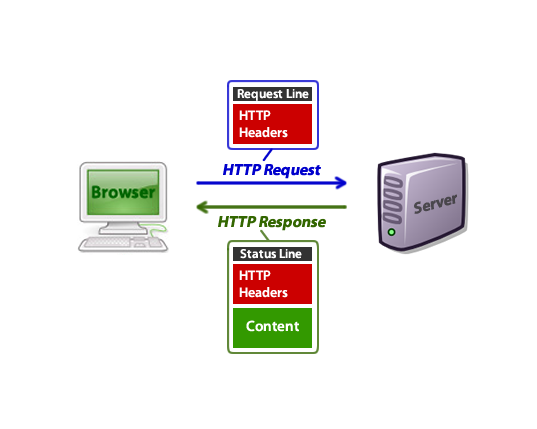
\includegraphics[scale=0.35]{http_diagram.png}
    	\caption{Diagramme des échanges HTTP (simplifié)}
    \end{figure}
\end{frame}
% Routing
\begin{frame}[fragile]
	\frametitle{HTTP: Le routage en quelques mots}
    
    Quant au routing, qui n'est pas une spécification propre à HTTP, mais plutôt un concept. Il s'agit d'associer à une URI (Uniform Resource Identifier), une ressource. \pause Exemple :
 
    \begin{verbatim}
    GET /meetups/python/everywhere HTTP/1.1
    Host: localhost:8000
    \end{verbatim}
\end{frame}
% Style REST
\begin{frame}[fragile]
	\frametitle{REST: Un style avant tout}
    
    REST est un style d'écriture d'API qui suit le standard HTTP, on le décrit comme :
    \pause
    \begin{itemize}[<+->]
    	\item HEAD/GET sont des opérations de lecture-seule et non dangereux.
        \item PUT/DELETE modifie une ressource.
        \item POST crée une nouvelle entité par rapport à l'URI.
        \item PATCH modifie une partie de l'entité.
    \end{itemize}
\end{frame}
% WSGI
\begin{frame}[fragile]
	\frametitle{WSGI: Une approche Python du web dev}
    
    Le WSGI (Web Server Gateway Interface) est une approche développé par Python afin de faire du dev web, en fait, ça se résume à :
    \pause
    \begin{itemize}[<+->]
    	\item Headers HTTP + méta-données placés dans un dictionnaire
        \item Le contenu du corps est stocké comme un flux (stream)
    \end{itemize}
\end{frame}
% 3. Aperçu de Falcon
\section{Aperçu de Falcon}
\begin{frame}[fragile]
	\frametitle{Hello, World!}
    \begin{minted}[gobble=4]{python}
    import falcon
    
    class ParisMeetup(object):
        def on_get(self, request, response):
            language = request.get_param('language')
            if not (language.lower() == "python"):
                raise falcon.exceptions.HTTPNotFound()
            
            response.body = "Paris.py 6 est en cours!"
            response.status = falcon.HTTP_200
                
    
    api = falcon.API()
    api.add_route('/paris/current_meetup', ParisMeetup())
    \end{minted}
\end{frame}
\begin{frame}[fragile]
	\frametitle{Faire une API}
    \pause
    Cela revient à : \mint{python}|zip(routes, ressources)|
    Or,
    \pause
    \begin{itemize}[<+->]
    	\item Une route : Une URI associée à une méthode HTTP
        \item Une ressource : Un \og{} crafteur \fg{} de réponse qui contient la logique de l'application
    \end{itemize}
\end{frame}
\begin{frame}[fragile]
	\frametitle{Un exemple plus complexe}
    
    Essayons de fabriquer une API qui permettrait de donner tous les meetups en cours sur un langage de programmation d'un endroit :
    \pause
    Par exemple, à Paris pour Python on a quoi$\ldots$
    \pause
    Faisons un design de l'API d'abord, on écrit les routes pour se donner un ordre d'idée de la forme qu'on aura :
    \pause
    \begin{verbatim}
    GET /meetups/language/place
    DELETE /meetups/language/place
    PUT /meetups/language/place
    \end{verbatim}
    \pause
    On aurait pu implémenter POST pour faire un nouveau meetup. Mais c'est laissé en exercice à l'audience !
\end{frame}
\begin{frame}[fragile]
	\frametitle{Un exemple plus complexe}
    
    On résume :
    \pause
    \begin{description}[<+->]
    	\item[GET] Ça sera pour savoir si il existe un meetup d'un langage (language) à un endroit (place). Cette méthode renverra du JSON contenant la liste, ou une erreur 404 si il n'existe \emph{aucun} meetup
        \item[DELETE] Ça sera pour supprimer un meetup
        \item[PUT] Cela sera utile pour changer des paramètres comme si le meetup se déroule ou les horaires du meetup. Ici, par abus de simplicité, on dira que ça consiste à dire que le meetup se déroule.
	\end{description}
\end{frame}
\begin{frame}[fragile]
	\frametitle{Un exemple plus complexe}
    
    \begin{minted}[gobble=4]{python}
    class MeetupResource(object):
    
        def __init__(self, meetup_db):
            self._db = meetup_db

        def on_get(self, request, response, ...):
            meetups = self._db.get(language, place)
            if meetups is None:
                raise falcon.exceptions.HTTPNotFound()
            response.content_type = 'application/json'
            response.body = json.dumps(meetups)
		
        ...
    \end{minted}
\end{frame}
\begin{frame}[fragile]
	\frametitle{Un exemple plus complexe}
    
    \begin{minted}[gobble=4]{python}
    class MeetupResource(object):
        ...
        
        def on_delete(self, request, response, ...):
            self._db.delete(language, place)
            response.status = falcon.HTTP_204

		...
     \end{minted}
\end{frame}

\begin{frame}[fragile]
	\frametitle{Un exemple plus complexe}
    
    \begin{minted}[gobble=4]{python}
    class MeetupResource(object):
        ...
        
        def on_put(self, request, response, ...):
            if not self._db.exists(language, place):
                raise falcon.exceptions.HTTPNotFound()

            self._db.set_running(language, place)
            if not (language.lower() == 'python'):
                response.status = falcon.HTTP_799   
        ...
    \end{minted}
\end{frame}

\begin{frame}[fragile]
	\frametitle{Un exemple plus complexe}
    
    \begin{minted}[gobble=4]{python}
    ...
    
    db = MockupDB()
    api = falcon.API()
    
    api.add_route('/meetups/{language}/{place}', 
                                MeetupResource(db))
    \end{minted}
\end{frame}
\begin{frame}[fragile]
	\frametitle{Testons!}
	
	\begin{minted}{console}
	gunicorn meetup:api
	\end{minted}
	\pause
	\begin{minted}{console}
	[5973] [INFO] Starting gunicorn 17.5
	[5973] [INFO] Listening at: http://127.0.0.1:8000 (5973)
	[5973] [INFO] Using worker: sync
	[5978] [INFO] Booting worker with pid: 5978
	\end{minted}
	
	\pause
	Mais$\ldots$ ? Comment on teste? C'est pas du HTML!
	
\end{frame}

% 4. Unit Test with Falcon
\section{Tester une API avec Falcon}
\begin{frame}[fragile]
	\frametitle{Le testing manuel}
    
	Souvent, on utilise \emph{curl} pour se faire ses petits tests. \pause \\
	Je vous propose \emph{httpie} :
	\pause
	\begin{itemize}[<+->]
		\item C'est basé sur \emph{python-requests}
		\item C'est human-friendly.
		\item Gestion du HTTP au top.
	\end{itemize}
	\pause
    \begin{minted}[gobble=4]{console}
    pip install httpie
    \end{minted}
\end{frame}
\begin{frame}[fragile]
	\frametitle{Alors, on teste?}
    
    \begin{minted}[gobble=4]{console}
    http get localhost:8000/meetups/c++/paris
    \end{minted}
    \pause
    \begin{verbatim}
    HTTP/1.1 200 OK
    Connection: close
    Date: Tue, 03 Feb 2015 21:29:44 GMT
    Server: gunicorn/17.5
    content-length: 23
    content-type: application/json

    {
        "name": "Paris.cpp 1"
    }
    \end{verbatim}
\end{frame}
\begin{frame}[fragile]
	\frametitle{Alors, on teste?}
    
    \begin{minted}[gobble=4]{console}
    http get localhost:8000/meetups/php/paris
    \end{minted}
    \pause
    \begin{verbatim}
    HTTP/1.1 404 Not Found
    Connection: close
    Date: Tue, 03 Feb 2015 21:30:44 GMT
    Server: gunicorn/17.5
    content-length: 0
    \end{verbatim}
\end{frame}
\begin{frame}[fragile]
	\frametitle{Alors, on teste?}
    
    \begin{minted}[gobble=4]{console}
    http delete localhost:8000/meetups/c++/paris
    \end{minted}
    \pause
    \begin{verbatim}
    HTTP/1.1 204 No Content
    Connection: close
    Date: Tue, 03 Feb 2015 21:32:53 GMT
    Server: gunicorn/17.5
    \end{verbatim}
\end{frame}
\begin{frame}[fragile]
	\frametitle{Et les tests unitaires, dans l'histoire?}
    C'est bien de tester manuellement parfois.
    Mais c'est inefficace à long terme :
    \pause
    \begin{itemize}
    	\item On doit forcément \alert{TOUT} tester pour \alert{prévenir la régression}, alors que des tests automatisés sont plus cools!
    \end{itemize}
    \pause
    Avec Falcon, on peut utiliser un helper de Falcon et carrément utiliser \emph{python-requests}.
\end{frame}
\begin{frame}[fragile]
	\frametitle{Les tests unitaires avec Falcon}
    Les développeurs Python habitués aux Unit Test utilisent le module \emph{unittest} en créant une classe, dérivant de \emph{unittest.TestCase} qui implémentera des tests automatiques.
\end{frame}
\begin{frame}[fragile]
	\frametitle{Reprenons nos exemples!}
    
    \begin{minted}[gobble=4]{python}
    import unittest
    import falcon.testing
    import meetup
    
    class MeetupTests(unittest.TestCase):
        def setUp(self):
        def tearDown(self):
        
        def simulate_request(self, path, **kwargs):
        
        def test_meetup_existence(self):
        def test_meetup_inexistence(self):
        def test_meetup_deletion(self):
        def test_method_not_allowed(self):
    \end{minted}
\end{frame}
\begin{frame}[fragile]
	\frametitle{Tests Unitaires: Configuration et nettoyage}
    
    \begin{minted}[gobble=4]{python}
    class MeetupTests(unittest.TestCase):
    
        def setUp(self):
            self.app = meetup.api
            self.mock = falcon.testing.StartResponseMock()
            self.paris_py_path = '/meetups/python/paris'
            self.paris_cpp_path = '/meetups/c++/paris'
            self.simulate_request(self.paris_py_path,
                method='POST', body='name=Paris.py 6')
            self.simulate_request(self.paris_cpp_path,
            	method='POST', body='name=Paris.cpp 1')
         
         ...
    \end{minted}
\end{frame}
\begin{frame}[fragile]
	\frametitle{Tests Unitaires: Configuration et nettoyage}
    
    \begin{minted}[gobble=4]{python}
    class MeetupTests(unittest.TestCase):
        ...
        
        def tearDown(self):
            self.simulate_request(self.paris_py_path,
            						   method='DELETE')
            self.simulate_request(self.paris_cpp_path,
            						   method='DELETE')
    \end{minted}
\end{frame}
\begin{frame}[fragile]
	\frametitle{Tests Unitaires: Simuler une requête}
    
    \begin{minted}[gobble=4]{python}
    class MeetupTests(unittest.TestCase):
        ...
        
        def simulate_request(self, path, **kwargs):
            env = falcon.testing.create_environ(
                path=path, **kwargs)
            return self.app(env, self.mock)
    \end{minted}
\end{frame}
\begin{frame}[fragile]
	\frametitle{Tests Unitaires: Les tests}
    
    \begin{minted}[gobble=4]{python}
   	class MeetupTests(unittest.TestCase):
        ...
        
        def test_meetup_existence(self):
            self.simulate_request(self.paris_py_path,
            							 method='GET')
            self.assertEqual(self.mock.status, 
            				   falcon.HTTP_200)
        
        def test_meetup_inexistence(self):
            self.simulate_request('/meetups/php/paris',
            							   method='GET')
            self.assertEqual(self.mock.status,
             				   falcon.HTTP_404)
        
        ...
    \end{minted}
\end{frame}
\begin{frame}[fragile]
	\frametitle{Tests Unitaires : Les tests}
    
    \begin{minted}[gobble=4]{python}
    class MeetupTests(unittest.TestCase):
    	...
        
        def test_meetup_deletion(self):
            self.simulate_request(self.paris_cpp_path,
            						   method='DELETE')
            self.assertEqual(self.mock.status,
            				   falcon.HTTP_204)
        
        def test_method_not_allowed(self):
            self.simulate_request(self.paris_py_path,
            						   method='PATCH')
            self.assertEqual(self.mock.status, 
            				   falcon.HTTP_405)
    \end{minted}
\end{frame}
\begin{frame}[fragile]
	\frametitle{Lancer les tests unitaires}
   	En Python, il existe plusieurs moyen de lancer des tests unitaires, le moyen de base est \emph{unittest} en exécutant le fichier contenant les tests.
   	\pause
    Ici, on utilisera \emph{nosetests} qui est une lib plus avancée que \emph{unittest} fourni de base\footnote{BATTERIES INCLUDED} avec Python :
    \pause
    \begin{minted}[gobble=4]{console}
    nosetests -v units_tests.py
    \end{minted}
    \pause
    \begin{verbatim}
    ....
    ---------------------
    Ran 4 tests in 0.162s

    OK
    \end{verbatim}
    
\end{frame}
% 5. Comparaison entre les autres lib (perfs & usages cases)
\section{Et les autres libs dans l'histoire?}
\begin{frame}{Pourquoi Falcon est né?}
	En réalité, on peut voir Falcon comme encore un nouveau framework mais pour reprendre les termes de l'auteur :
	\pause
    \begin{itemize}[<+->]
    \item Les frameworks web Python actuels n'ont pas des \emph{perfs géniales} lorsqu'ils sont soumis à des \alert{grosses charges}. 
    \item La plupart des framework sont embarqués en fait avec des lib de templating, des fonctionnalités shiny qui sont \alert{utiles} uniquement lorsqu'on fait un site. Elles peuvent augmenter la chance de \alert{faille de sécurité}, gâchent de la RAM.
    \end{itemize}
    \pause
	La \emph{raison d'être} de Falcon est de \emph{résoudre} ces problèmes.
\end{frame}
\begin{frame}{Mais Falcon n'est pas la solution ultime}
	Certes, Falcon est vraiment bon pour faire des API. Mais ce n'est pas le meilleur choix partout :
	\pause
    \begin{description}[<+->]
    	\item[DRY] Si vous switchez entre votre web app et votre API en changeant de framework systématiquement, ça n'a pas de sens. Il est plus intéressant de prendre un framework \emph{moins spécialisé}.
        \item[Usine à gaz] Falcon est tout sauf une usine à gaz, donc, il faut se préparer à produire des lignes de plus en échange d'une plus grande liberté. Pour le \alert{Quick \& Dirty}, il faudra aller voir Flask/Django, etc.
        \item[Maturité] Falcon est un projet né en 2013. Il a \emph{moins} été \alert{testé sur le terrain} que ses grands frères dans le domaine.
    \end{description}
\end{frame}

\begin{frame}{Un petit benchmark}
	\begin{table}
        \caption{Comparatif sous Python 2.7.6}
        \pause
    	\begin{tabular}{llrrr}
          \toprule
          Frameworks & Type & requêtes/s & µs/requêtes & Performance \\
          \midrule
          Falcon (0.1.8) & Simple & 24 358 & 41 & 8x \\
          Falcon (0.1.8) & Étendu & 17 787 & 56 & 6x \\
          Bottle (0.11.6) & Simple & 13 623 & 73 & 4x \\
          Werkzeug (0.9.4) & Simple & 5 163 & 194 & 2x \\
          Flask (0.10.1) & Simple & 3 041 & 329 & 1x \\
          \bottomrule
        \end{tabular}
    \end{table}
\end{frame}

% 6. Résumé & conclusion
\section{Conclusion}
\begin{frame}{Résumé}
	Falcon est un choix intéressant pour une API aujourd'hui :
    \pause
    \begin{itemize}[<+->]
    	\item On fait de plus en plus de sites avec des frameworks frontend JavaScript qui fetch des données \alert{d'une API}.
        \item La \alert{productivité} que permet Falcon.
        \item Sa \alert{rapidité} en général.
    \end{itemize}
\end{frame}

\begin{frame}{A propos des slides}
	Ces slides ont été faits en \LaTeX{}, vous pouvez retrouver le code source sur GitHub (ainsi que la petite API) dans le repo suivant :
	
    \begin{center}\url{github.com/RaitoBezarius/falcon-introduction}\end{center}
    
    En licence WTFPL\footnote{J'avais pas d'idées lorsque j'allais l'open-sourcer}, naturellement.
    
    Le thème beamer utilisé est le mtheme (disponible sur GitHub) fait par Matthias Vogelgesang (matze sur Github).

\end{frame}

\plain{Questions?}
\plain{Merci à tous d'avoir assisté à cette présentation!}

\end{document}